\documentclass{article}
\usepackage[final]{nips_2017}
\usepackage[utf8]{inputenc} % allow utf-8 input
\usepackage[T1]{fontenc}    % use 8-bit T1 fonts
\usepackage{hyperref}       % hyperlinks
\usepackage{url}            % simple URL typesetting
\usepackage{booktabs}       % professional-quality tables
\usepackage{amsfonts}       % blackboard math symbols
\usepackage{nicefrac}       % compact symbols for 1/2, etc.
\usepackage{microtype}      % microtypography
\usepackage{graphicx}
\usepackage[font=small, labelfont=bf]{caption}
\usepackage{subcaption}
\usepackage{float}
\usepackage{amsmath}
\usepackage{natbib}
\usepackage{tabularx}

\title{Graph Convolutional Network in Classifying Rock Climbing Difficulties}

\author{
  Cheng-Hao Tai \\
  Microsoft Corporation \\
  Stanford University \\
  \texttt{c2tai@stanford.edu} \\
  \And
  Aaron Wu \\
  Evisort Inc. \\
  - \\
  \texttt{aaron@evisort.com} \\
  \And
  Rafael Hinojosa \\
  Microsoft Corporation \\
  Stanford University \\
  \texttt{rahinojo@stanford.edu} \\
}

\begin{document}

\begin{center}

\includegraphics[width=3cm, height=0.7cm]{CS230}
\end{center}

\maketitle

\begin{abstract}
The abstract should consist of 1 paragraph describing the motivation for your paper and a high-level explanation of the methodology you used/results obtained.
\end{abstract}

\section{Introduction}	
Given rock climbing's considerable popularity, we created a neural network for classifying climbing routes (a.k.a. problems) into suitable difficulty categories. This tool could either speed up or replace traditionally heuristic-based approachs to ranking climbing problems, thereby lowering the barrier of entry for anyone seeking to create their own routes. We solved this problem using a classifier built for the "Moonboard" apparatus --- a modular climbing wall of fixed dimensions and pre-set hold configurations (Figure 1) and took inspiration from the NLP domain where Graph Convolutional Network architectures have demonstrated great success in document classification tasks.

{\small\textbf{Our codebase can be found here: \texttt{https://github.com/gestalt-howard/moonGen}}}

\section{Related Works}
Existing machine learning literature for rock climbing is sparse and primarily utilizes Bayesian approaches towards categorizing route difficulties. The earliest attempt of its kind was in 2012 \cite{Phillips_2012} where the authors applied chaos theory in conjunction with a Variational-Order Markov Model to first generate, then classify climbing routes. More recently, \cite{scarff2020estimation} presented a novel application of Whole-History Rating (WHR) \cite{RemiCoulomWHR} to determine route difficulties based on historical user ratings. As far as we're aware, \cite{DoblesCS229} is the first to apply deep learning (using a convolutional neural network) in classifying route difficulty.

Looking outside of climbing-specific literature, many inspirations can be drawn from the NLP field --- specifically text classification --- through the observation that just as words constitute sentences, rock climbing problems are composed of holds. In 2018, Cer et al. \cite{cer2018universal} demonstrated the power of robust sentence embeddings in solving text classification tasks. In their paper, Cer et al. utilized an attention mechanism to capture contextual relationships of words in a sentence to generate weights subsequently used to aggregate word vectors into sentence encodings. 

Using a graph neural network \cite{battaglia2018relational}, it is possible to explicitly encode the aforementioned attention weights through edge weights in an adjacency matrix. In \cite{kipf2016semisupervised}, Kipf et al. presents the graph convolutional network architecture that is expanded upon by Yao et al. in \cite{yao2018graph} for a text classification task on a heterogenous graph of document / word nodes.

\section{Dataset and Features}
On their website (\texttt{https://moonboard.com}), Moonboard hosts a database of Moonboard climbing routes, created and ranked by a global climbing community. For a given hold configuration (i.e. Moonboard 2016), routes are denoted using multi-colored circles superimposed on a stock Moonboard image. These circles specify a hold set and define a problem: green, blue, and red circles indicate starting, intermeidate, and end positions, respectively (Figure 1). MoonBoard 2016 has exactly 140 holds.

Assembling this dataset required a custom Selenium scraping script that clicked through thousands of pages of Moonboard problems, stopping on each page to extract metadata tags, labels, and features. The data is separated into 15 distinct difficulty categories denoted as V4 through V14 with ascending numerical values corresponding to increasing route difficulty. By its nature, our dataset is highly imbalanced with V4 and V5 routes accounting for over 50\% of 13,589 problems while V11 through V14 contribute approximately 1\%. To counteract this extreme data imbalance, we implemented a balanced sampling protocol that upsamples sparse classes and ensures that each difficulty category is equally-represented during model training.

MoonBoard problem data were further preprocessed into either one-hot or multi-hot representations. In its multi-hot form, each MoonBoard is represented as a 140-dimensional vector with each dimension encoding presence / absence of one of the 140 holds. A PCA-decomposed 2D visualization of the problem corpus is shown in Figure 1.

\begin{figure}[h]
\centering
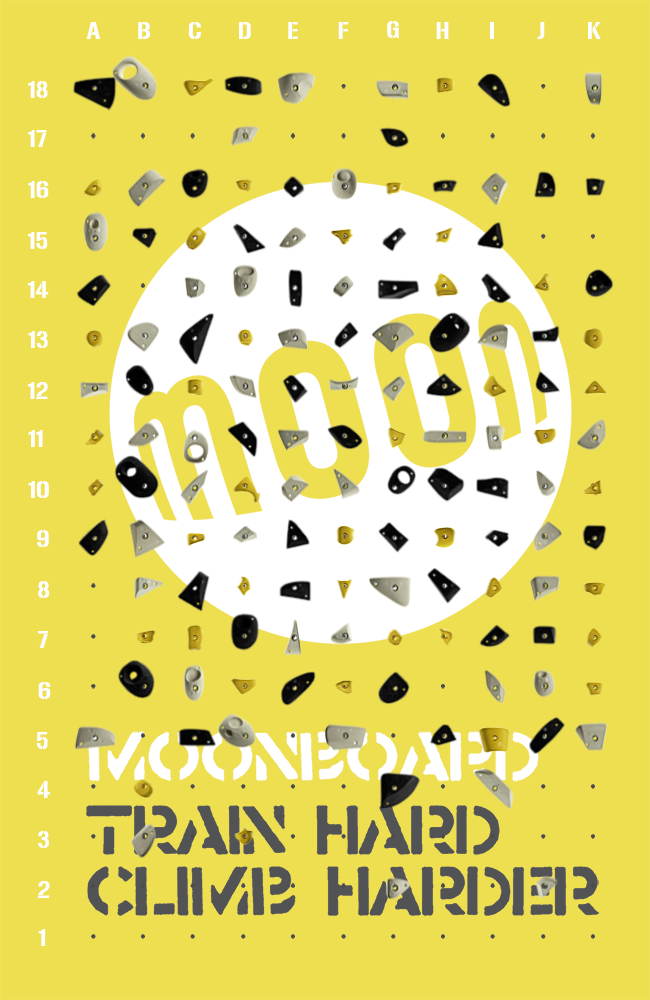
\includegraphics[width=.255\textwidth]{moonboard_stock}\hfill
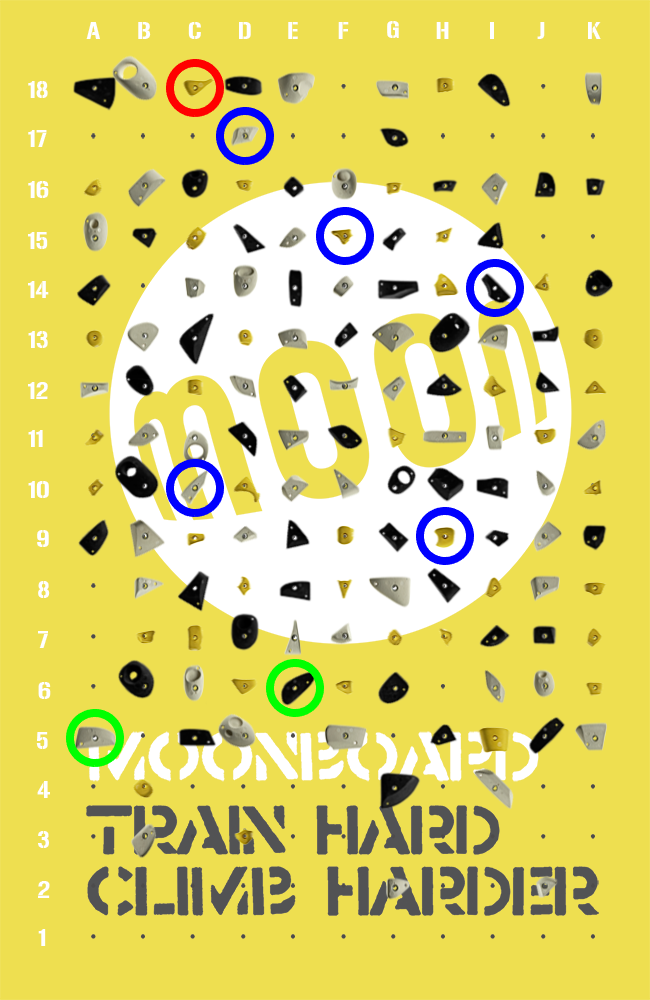
\includegraphics[width=.255\textwidth]{moonboard_1}\hfill
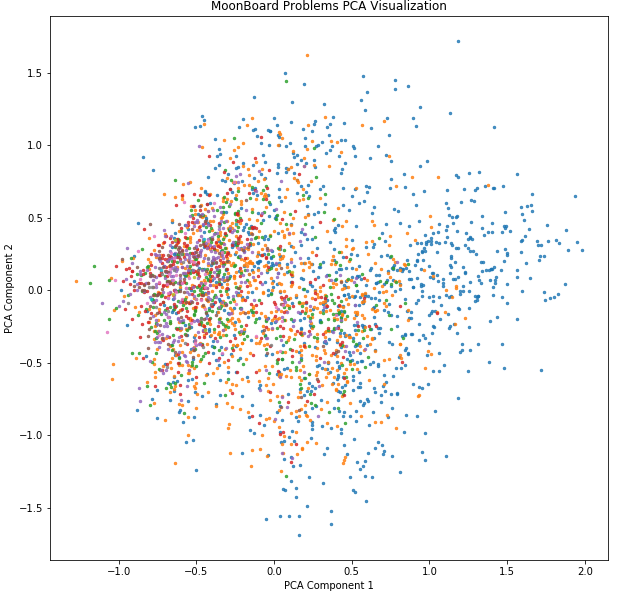
\includegraphics[width=.43\textwidth]{pca_visual}

\label{fig: MoonBoard data description}
\caption{(left) MoonBoard stock configuration (version 2016), (center) A specific MoonBoard route on the 2016 configuration, (right) Visualization of PCA decomposition of MoonBoard problems}
\end{figure}

\section{Methods}

\subsection{Graph Convolutional Network}
The Graph Convolutional Network as presented by \cite{kipf2016semisupervised} provides a framework by which node-level features can be combined with neighbors in a nonlinear transformation whose parameters are learned through backpropagation. Consider a graph $G = (V,E)$ where $V(\lvert V\rvert\ = n)$ and $E$ are the set of nodes and edges, respectively. Each node in $V$ is assumed to be connected to itself (self-adjacency) and is represented as a row in $X \in \mathbb{R}^{n \times m}$. Graph $G$ also has an adjacency matrix $A$ with a corresponding degree matrix $D$ where $D_{ii} = \sum_{j}A_{ij}$. A one-layer GCN featuring 1 convolution step is computed as
\begin{equation}
L^{1} = \rho(\widetilde{A}XW_{0})
\end{equation}
where $\widetilde{A} = D^{-\frac{1}{2}}AD^{-\frac{1}{2}}$ is the normalized symmetric adjacency matrix, $W_0 \in \mathbb{R}^{m \times k}$ is a weight matrix, and $\rho$ is an activation function. This one-step convolutional operation captures information about a node's immediate neighbors. 

\begin{figure}
\centering
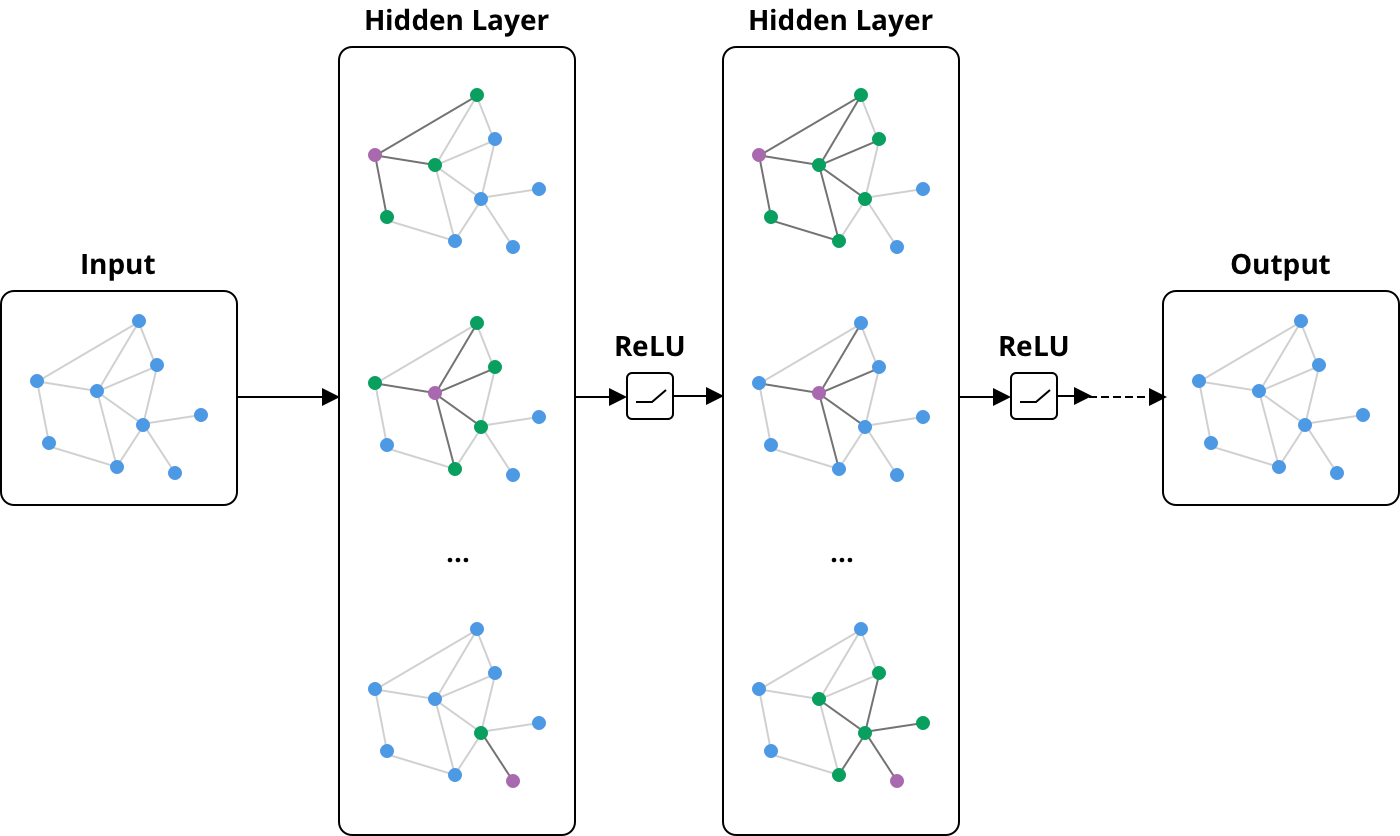
\includegraphics[width=.5\linewidth]{gcn_2steps}
\caption{At the first convolutional step, any node has access to its 1-hop neighbors. At the second convolution, nodes can "see" features from their 2-hop neighbors. Generally, $k$ convolution steps yields access to features from $k$-hop neighbors.}
\label{fig: Graph Convolutional Network}
\end{figure}

\begin{figure}
\centering
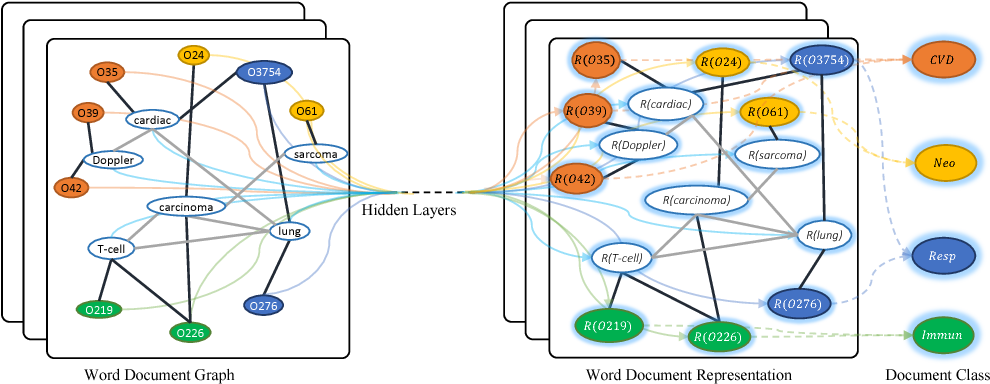
\includegraphics[width=.6\linewidth]{textGCN}
\caption{A heterogenous corpus graph for document classification using a Text GCN \cite{yao2018graph}. Nodes come in 2 types: document entities and word entities. The different colors correspond to different node categories (notice only document nodes are colored). A direct analogy to Moonboard problems can be made by substituting documents for problems and holds for nodes.}
\label{fig: Corpus graph for Text Graph Convolutional Network}
\end{figure}

\subsection{Defining Adjacency}

\begin{equation}
A_{ij}= 
\begin{cases}
    \text{PMI}(i, j), & \text{if } i, j \text{ holds} \\
    \text{IDF}(j), & \text{if } i \text{ problem } j \text{ hold} \\
    1, & \text{if } i=j \\
    0, & \text{otherwise}
\end{cases}
\end{equation}

In the above equation, \texttt{PMI} refers to \textit{Pointwise-Mutual Information} --- a metric that measures the degree of independence between two random variables and in our context can be interpreted as the log co-occurrence probability of holds. \texttt{IDF} refers to the \textit{Inverse Document Frequency} component of the famous \texttt{TFIDF} embedding strategy. While the authors of [3] used TFIDF in defining adjacency between words and documents, term frequency is redundant in our context since holds can never appear more than once in a single Moonboard route.

On the modeling side, we've implemented a baseline logistic regression classifier using feature set (2) along with a preliminary PyTorch implementation of the Text GCN [3] architecture using feature set (1) --- both models utilizing multi-class cross-entropy loss. Referencing Figure 1 which reports the baseline logistic regression model's performance metrics, we can see that this classification task is possible even for a simple LR model --- giving us confidence in continuing down the GCN route.

\section{Experiments, Results, and Discussions}

% Table of results
\begin{table}[h!]
\centering
\caption{Summary of experiment results with per-class F1 scores and averaged accuracy, F1, and AUC scores}
\label{tab:my-table}
\begin{tabular}{@{}lccclccccc@{}}
\toprule
                            & \multicolumn{7}{c}{\textbf{Per-Class F1 Scores}} & \multicolumn{2}{c}{\textbf{Avg.}} \\ \midrule
\textbf{Experiment} & \textbf{V4} & \textbf{V5} & \textbf{V6} & ... & \textbf{V12} & \textbf{V13} & \textbf{V14} & \textbf{F1} & \textbf{AUC} \\
Logistic Regression         & 0.52  & 0.35  & 0.25  & ... & 0.22 & 0.00 & 0.00 & 0.23            & 0.70            \\
SVM                         & 0.53  & 0.40  & 0.31  & ... & 0.34 & 0.33 & 0.00 & 0.29            & 0.66            \\
Random Forest               & 0.66  & 0.36  & 0.26  & ... & 0.24 & 0.00 & 0.44 & 0.28            & 0.67            \\
Gradient Boosting           & 0.59  & 0.35  & 0.28  & ... & 0.27 & 0.25 & 0.00 & 0.27            & 0.62            \\
MLP                         & 0.58  & 0.38  & 0.34  & ... & 0.00 & 0.00 & 0.00 & 0.22            & 0.66            \\
Dense Shallow, MH           & 0.61  & 0.38  & 0.32  & ... & 0.37 & 0.00 & 0.00 & 0.26            & 0.67            \\
Dense Deep, MH              & 0.48  & 0.40  & 0.23  & ... & 0.21 & 0.00 & 0.00 & 0.22            & 0.65            \\
GCN (S) 2S, OH, PMI         & 0.36  & 0.28  & 0.22  & ... & 0.48 & 0.24 & 0.10 & 0.24            & 0.63            \\
GCN (L) 2S, OH, PMI         & 0.33  & 0.27  & 0.23  & ... & 0.48 & 0.25 & 0.13 & 0.24            & 0.64            \\
GCN (S) 2S, MH, PMI         & 0.57  & 0.38  & 0.33  & ... & 0.49 & 0.00 & 0.00 & 0.29            & 0.73            \\
GCN (L) 2S, MH, PMI         & 0.58  & 0.38  & 0.33  & ... & 0.45 & 0.00 & 0.00 & 0.29            & 0.72            \\
GCN (S) 2S, MH, Binary      & 0.54  & 0.38  & 0.33  & ... & 0.46 & 0.00 & 0.00 & 0.28            & 0.72            \\
GCN (S) 2S, MH, Self-Binary & 0.58  & 0.41  & 0.30  & ... & 0.14 & 0.00 & 0.00 & 0.25            & 0.70            \\
GCN (S) 2S, MH, Self-PMI    & 0.59  & 0.38  & 0.29  & ... & 0.56 & 0.00 & 0.00 & 0.27            & 0.68            \\
GCN (L) 4S, MH, PMI         & 0.52  & 0.34  & 0.33  & ... & 0.50 & 0.00 & 0.37 & 0.31            & 0.73            \\
GCN (S) 2S, MH, Win-PMI     & 0.55  & 0.37  & 0.33  & ... & 0.48 & 0.00 & 0.00 & 0.28            & 0.73            \\
GCN (L) 2S, MH, Win-PMI     & 0.57  & 0.38  & 0.34  & ... & 0.47 & 0.00 & 0.00 & 0.29            & 0.72            \\ \bottomrule
\end{tabular}
\end{table}

To guide our decision-making throughout the remainder of this project, we invested significant effort in creating robust, custom evaluation metrics for monitoring model performance. Since our objective is multi-category classification, our evaluation strategy incorporates many proven classification-compatible metrics (i.e. F1-score, accuracy, recall, precision, AUC) along with confusion matrices and correlation plots. In addition, we extended each of these techniques to accomodate a sliding window over the difficulty classes. This custom addition encodes an intuition that we are willing to accept a \(+/- 1\) margin of error in our difficulty classification (i.e. a V4 problem can be mistaken for a V5 but not a V6, if using a sliding window size of 1). Altogether, these metrics are combined into three distinct visualizations (see Table 1) 

\begin{figure}
\centering
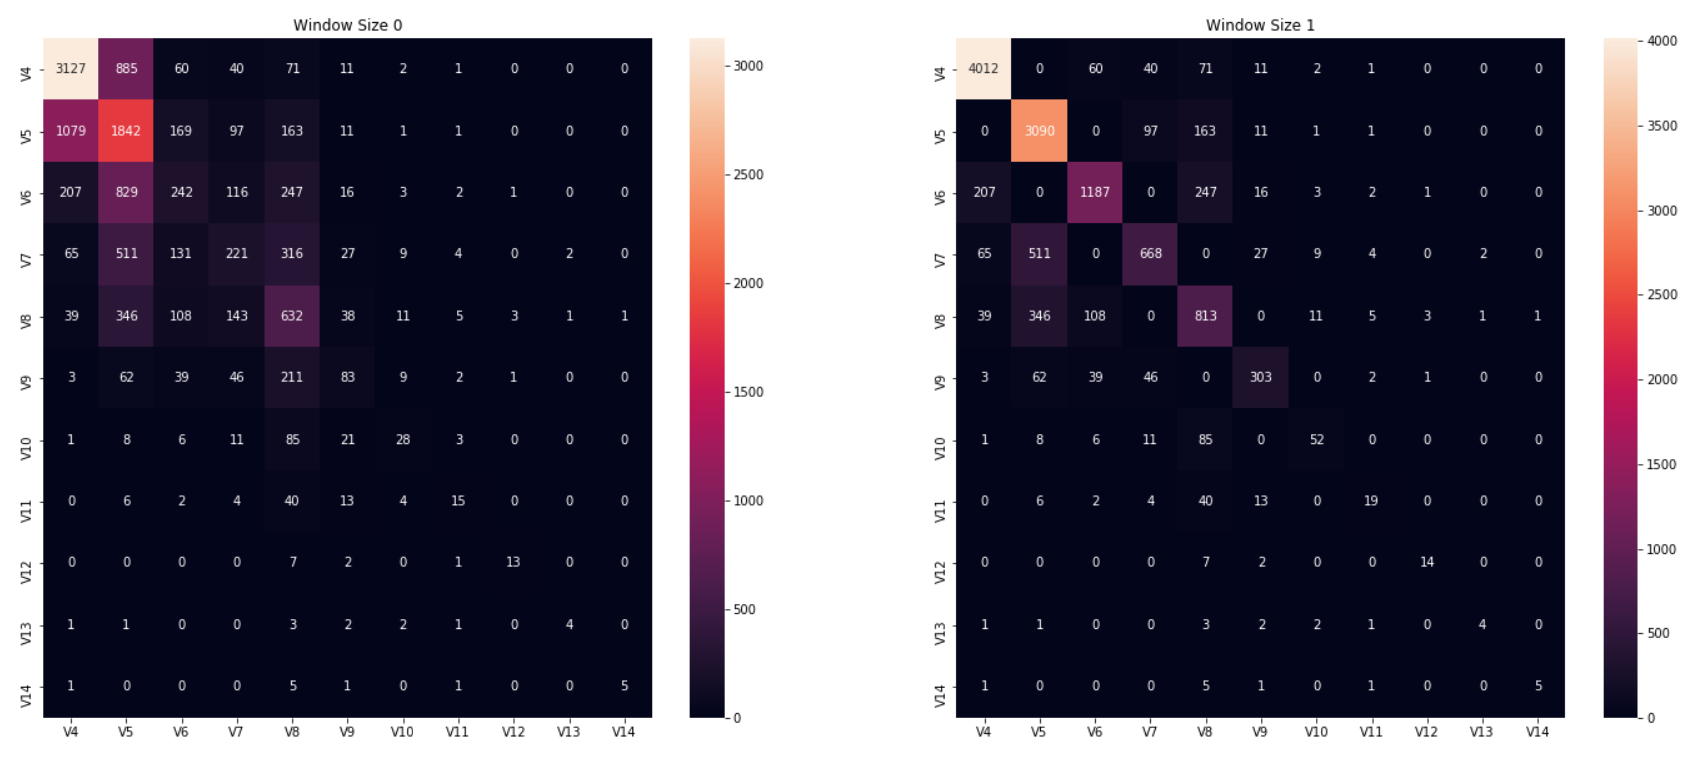
\includegraphics[width=.8\linewidth]{confusion_window}
\caption{Two confusion matrices that present a novel approach to model evaluation of a multi-category classifier. The left-hand plot shows a vanilla confusion matrix implementation (Window Size 0) while the right-hand matrix incorporates a sliding-window approach (Window Size 1) to determining false positive / true positive rates amongst the different difficulty classes.}
\end{figure}

\section{Conclusions / Future Work}
We plan on continuing to refine our GCN implementation by evaluating performance under different feature sets and adjacency definitions such that we are able to thoroughly characterize the behavior of our GCN model. Should we have additional time, we will explore a generative application [1] capable of producing a new Moonboard problem, given a user-specified difficulty.

\section{Contributions}

\bibliographystyle{plain}
\bibliography{citations}

\end{document}